%%%%%%%%%%%%%%%%%%%%%%%%%%%%%%%%%%%%%%%%%%%%%%%%%%%%%%%%%%%%%%%%%%%%%%%%%%%%%%%%
%2345678901234567890123456789012345678901234567890123456789012345678901234567890
%        1         2         3         4         5         6         7         8

\documentclass[letterpaper, 10 pt, conference]{ieeeconf}  % Comment this line out if you need a4paper

%\documentclass[a4paper, 10pt, conference]{ieeeconf}      % Use this line for a4 paper

\IEEEoverridecommandlockouts                              % This command is only needed if 
                                                          % you want to use the \thanks command

\overrideIEEEmargins                                      % Needed to meet printer requirements.

%In case you encounter the following error:
%Error 1010 The PDF file may be corrupt (unable to open PDF file) OR
%Error 1000 An error occurred while parsing a contents stream. Unable to analyze the PDF file.
%This is a known problem with pdfLaTeX conversion filter. The file cannot be opened with acrobat reader
%Please use one of the alternatives below to circumvent this error by uncommenting one or the other
%\pdfobjcompresslevel=0
%\pdfminorversion=4

% See the \addtolength command later in the file to balance the column lengths
% on the last page of the document

% The following packages can be found on http:\\www.ctan.org
\usepackage{graphics} % for pdf, bitmapped graphics files
\usepackage{epsfig} % for postscript graphics files
\usepackage{mathptmx} % assumes new font selection scheme installed
\usepackage{times} % assumes new font selection scheme installed
\usepackage{amsmath} % assumes amsmath package installed
\usepackage{amssymb}  % assumes amsmath package installed
\usepackage{mathtools}
\usepackage{relsize}
\usepackage{tikz}
\graphicspath{{./Drawings/}} 
\newcommand{\notimplies}{%
	\mathrel{{\ooalign{\hidewidth$\not\phantom{=}$\hidewidth\cr$\implies$}}}}
\usepackage[margin=0.8cm]{caption}
\newcommand{\norm}[1]{\left\lVert#1\right\rVert}
\usepackage{pgfplots}
\pgfplotsset{compat=newest}
\pgfplotsset{plot coordinates/math parser=false}
\newlength\figureheight
\newlength\figurewidth 
\usepackage{adjustbox}
\usepackage{indentfirst}

\newtheorem{lemma}{Lemma}
\newtheorem{theorem}{Theorem}


\setlength{\parindent}{15pt} % Default is 15pt.
\newcommand{\AB}[1]{\textbf{\color{magenta}{[AB: #1]}}}
\newcommand{\SK}[1]{\textbf{\color{blue}{[SK: #1]}}}
\newcommand{\smallmat}[1]{\left[ \begin{smallmatrix}#1 \end{smallmatrix} \right]}

\title{\LARGE \bf
Robustified data-driven model predictive control
}


\author{Sampath Kumar Mulagaleti$^{1}$ and Alberto Bemporad$^{2}$% <-this % stops a space
\thanks{*This work was not supported by any organization}% <-this % stops a space
\thanks{$^{1}$Albert Author is with Faculty of Electrical Engineering, Mathematics and Computer Science,
        University of Twente, 7500 AE Enschede, The Netherlands
        {\tt\small albert.author@papercept.net}}%
\thanks{$^{2}$Bernard D. Researcheris with the Department of Electrical Engineering, Wright State University,
        Dayton, OH 45435, USA
        {\tt\small b.d.researcher@ieee.org}}%
}

\bibliographystyle{ieeetr}
\begin{document}



\maketitle
\thispagestyle{empty}
\pagestyle{empty}


%%%%%%%%%%%%%%%%%%%%%%%%%%%%%%%%%%%%%%%%%%%%%%%%%%%%%%%%%%%%%%%%%%%%%%%%%%%%%%%%
\begin{abstract}

This paper presents a robust data-driven control approach for linear systems subject to bound constraints on inputs and outputs.
 The approach builds on a previously presented hierarchical direct data-driven control architecture for constrained systems. Improved robustness is achieved by using a robust model predictive controller (RMPC) instead of a deterministic model predictive controller (MPC) in the outer loop of the architecture. The RMPC controller generates a reference signal for the inner loop under robust constraints based on a model of the inner loop and a bounded disturbance set. A major contribution of this work is the development of a method to calculate the disturbance set from an identified AutoRegressive model with eXogenous inputs (ARX). We validate numerically the robustified control architecture, showing significant improvements with respect to its deterministic counterpart.

\end{abstract}


%%%%%%%%%%%%%%%%%%%%%%%%%%%%%%%%%%%%%%%%%%%%%%%%%%%%%%%%%%%%%%%%%%%%%%%%%%%%%%%%
\section{Introduction}
Design of control systems can be broadly classified into two categories: \emph{model-based} and \emph{model-free}. Model-based control design techniques use an explicit model of the plant being controlled, derived from physical principles or identified from data. This involves selecting a model that trades-off between complexity and accuracy. Model selection is followed by experiments to identify the parameters. These steps introduce several challenges, that one
can avoid by resorting to a ``direct'' data-driven controller design methodology.

Direct data-driven controller design methods avoid explicitly identifying the plant model, so that we can label them as ``model free''. They synthesize a controller directly from I/O data obtained from the plant. A review of several such methods can be found in \cite{HOU20133}. One such method, virtual reference feedback tuning (VRFT) introduced in \cite{CAMPI20021337}, has been used to design a stabilizing feedback controller within a hierarchical control architecture in \cite{7932940} for LTI/LPV systems. The architecture employs an outer MPC controller, which utilizes the reference model selected for VRFT to generate a tracking signal. Performance bounds on the plant are translated into constraints on the optimization problem solved by the MPC controller. Since the reference model might not reasonably reflect the performance of the closed-loop plant, there is the possibility of violating the constraints imposed on input/output variables. 

It is therefore desirable to use a robust MPC controller in the outer loop, which generates a tracking signal that robustly satisfies the system constraints. A review of the concepts related to robust MPC controllers can be found in \cite{10.1007/BFb0109870}. An alternative is to use a robust reference governor, which modifies the reference signal supplied to the plant in a way that constraints are satisfied~\cite{GARONE2017306}. Both techniques not only need a model of the \emph{closed-loop} system, but also a model of the associated uncertainties.

In this work, we propose a data-driven control approach with improved robustness properties.
We build on the hierarchical control architecture presented in \cite{7932940}. The robust controller uses a model with uncertainty of the inner closed-loop, which consists of the plant and the VRFT-based feedback controller. This model consists of the reference model used for VRFT appended with an ARX model describing the uncertainty. The latter is identified from closed-loop experiments. 

The model incorporates uncertainties as exogenous disturbance signals, assumed to lie within an unknown bounded polyhedral set. Since robust control methods explicitly incorporate uncertainty information in their formulation, identification of the polyhedral uncertainty sets is necessary.

We propose a novel method to calculate the polyhedral sets of the exogenous disturbance signals. Such a method falls under the umbrella of identification for robust control.
This field includes a large volume of literature on set-membership techniques for parameter estimation. A review of these can be found in \cite{WALTER1990449}. A method to obtain ellipsoidal parameterizations of these sets during ARX estimation is discussed in \cite{7330793}. To the best of the authors' knowledge, no similar work has been done to calculate polyhedral sets of input exogenous disturbance signals from output data.

Following the identification of a model and corresponding disturbance sets, an RMPC controller is then designed, which replaces the deterministic MPC controller in the outer loop of the hierarchical architecture presented in \cite{7932940}.

The paper is organized as follows. In Sect. \ref{Problem statement}, the problem is formally stated. Background regarding the hierarchical data-driven control architecture and proposed robust model predictive controller is presented in Sect. \ref{Background}. Sect. \ref{Contribution} presents the techniques used to identify the model of the closed-loop system with disturbance bounds, which is the main contribution of this paper. Finally, Sect. \ref{Case studies} presents a numerical example implementing the robust hierarchical control design approach. 

\section{Problem statement}
\label{Problem statement}
We consider, for simplicity, a \textit{single-input single-output} (SISO) system $\mathbb{G}_P$ (unknown and not recovered from data) generating an output signal $y(t) \in \mathbb{R}$ corresponding to the input signal $u(t) \in \mathbb{R}$, $t \in \mathbb{Z}^+$. We aim at synthesizing a controller that can make $y(t)$ accurately track any user-defined reference signal, while satisfying the constraints
\begin{equation} 
\begin{array}{l}
y_{min}\leq y(t) \leq y_{max}\\
u_{min}\leq u(t) \leq u_{max},\quad t=0,1,\ldots
\end{array}
\label{constraints}
\end{equation} 
Following the direct data-driven controller synthesis methodology, we use the dataset $D_{N}=\{u(t),y(t);t\in{1,...,N}\}$ obtained by exciting the system to design the controller. %\footnote{We do not discuss here how to properly excite the system.}.

\section{Background}
\label{Background}
\subsection{Hierarchical approach}
A feedback controller is designed to control the system, using the VRFT methodology. For this, a reference model $\mathbb{M}_P$ is selected, given by:
	\begin{equation*}
\begin{array}{rcl}
	x_M(t+1) &=& A_Mx_M(t) + B_Mg(t)\\
	y_M(t) &=& C_Mx_M(t)
\end{array}
	\end{equation*}
For an approach to how to choose $\mathbb{M}_P$ optimally the reader is referred
to the recent work~\cite{SPB18}.
Using the VRFT methodology, we design a linear feedback controller $\mathbb{K}_P$, with the goal of making the closed-loop system $\mathbb{K}_P$-$\mathbb{G}_P$ behave similar to the reference model $\mathbb{M}_P$. Note that the model $\mathbb{G}_P$ is unknown and not needed by the procedure, which is therefore a model-free one. %It utilizes the dataset $D_N$ for controller synthesis. 
The steps of the VRFT approach for synthesizing $\mathbb{K}_P$ are summarized below:
\begin{enumerate}
	\item
	Use the dataset $D_N$, set $y_M(t)=y(t)$, calculate the virtual reference input $g(t)$ by by inverting the model $\mathbb{M}_P$, i.e, $g(t) = \mathbb{M}_P^{\dagger}y(t)$;
	\item
	Parameterize the feedback controller $\mathbb{K}_P$ as $A_K(q^{-1})u(t) = B_K(q^{-1})(g(t)-y(t))$, where 
	\begin{equation*}
	\begin{matrix}
	A_K(q^{-1}) = 1+\mathlarger{\sum\limits_{i=1}^{n_{a_K}}}a_i^Kq^{-i}\\
	B_K(q^{-1}) = \mathlarger{\sum\limits_{i=1}^{n_{b_K}}}b_i^Kq^{-i};
	\end{matrix}  
	\end{equation*}
	\item Use system identification to estimate the coefficients $a_i^K$ and $b_i^K$, e.g., via least-squares:
	\begin{equation}
	\small
	\begin{aligned}
	 \underset{a_i^K,b_i^K}{\text{min}}
	 & \hspace{5pt} \frac{1}{N}\mathlarger{\sum\limits_{t=1}^N}\mathlarger{\mathlarger{(}}A_K(q^{-1})u(t)-B_K(q^{-1})(\mathbb{M}_P^{\dagger}y(t)-y(t))\mathlarger{\mathlarger{)}}^2.
	\end{aligned}
	\label{VRFT_problem}
	\end{equation}
	\normalsize
\end{enumerate}
Problem~\eqref{VRFT_problem} minimizes the deviation between the control input calculated by the controller and the signal $u(t)$ that was used to excite the system and obtain $y(t)$.
\begin{figure}[t]
		\hspace{30pt}
	\includegraphics[scale=0.8]{KpGp.pdf}
	\caption{Feedback controller designed using VRFT}
\end{figure}
To satisfy plant constraints, the reference signal $g(t)$ is generated using an MPC controller in an outer loop. The objective of the MPC controller is to make the output signal $y(t)$ track an arbitrary reference $r(t)$ while satisfying constraints on $y(t)$ and $u(t)$. This is achieved by taking $\mathbb{M}_P$ and $\mathbb{K}_P$ as prediction model with 
output $[y(t),u(t)]$, that we denote as $\mathbb{M}'_P$:
	\begin{equation*}
	\begin{matrix}
	\zeta(t+1) = A_\zeta\zeta(t) + B_\zeta g(t)\\
	\begin{bmatrix}y(t)\\u(t)\end{bmatrix} = C_\zeta\zeta(t) + D_\zeta g(t)
	\end{matrix}
    \label{eq:cl-model}
	\end{equation*}
At each time step $t$ MPC solves the following optimal control problem over a horizon of $N_P$ steps
	\begin{equation}
	\small
	\begin{aligned}
	 \underset{\{g(t+k)\}_{k=1}^{N_P}}{\text{min}}
	& \hspace{20pt} Q_y\mathlarger{\sum\limits_{k=1}^{N_P}}(y(t+k|t)-r(t+k))^2 + Q_{\epsilon}\epsilon^2 \\
	 \text{subject to}
	&   \hspace{20pt}
	\zeta(t+k+1) = A_\zeta\zeta(t+k) + B_\zeta g(t+k)\\
	& \hspace{20pt} \begin{bmatrix}y(t+k)\\u(t+k)\end{bmatrix} = C_\zeta\zeta(t+k) +  \begin{bmatrix}0\\D_\zeta\end{bmatrix}g(t+k)\\
	& \hspace{20pt}  y_{min}-V_y\epsilon \leq y(t+k) \leq  y_{max}+V_y\epsilon \\
	& \hspace{20pt}  u_{min}-V_u\epsilon \leq u(t+k) \leq u_{max}+V_u\epsilon \\
	& \hspace{20pt}  \zeta(t|t) = \zeta(t)
	\end{aligned}
	\label{MPC}
	\end{equation}
	\normalsize
	The quantities $V_y$ and $V_u$ in the MPC formulation are used as soft constraints to avoid infeasibility of the optimization problem over successive iterations, since the reference model $\mathbb{M}'_P$ might not accurately capture the dynamics of the closed loop $\mathbb{K}_P-\mathbb{G}_P$. This implies that constraint satisfaction is not guaranteed by the data-driven approach~\cite{7932940} recalled above. 
	
	\subsection{Robustified model predictive controller}
\AB{I changed the formulation completely, I suspect the previous one was not correct}.

	To improve constraint satisfaction, the deterministic MPC controller in the outer loop of the hierarchical control architecture is replaced by a robust MPC (RMPC) controller. A schematic of the control loop is shown in Figure \ref{fullloop}. 
	\begin{figure}[t]
		\vspace{-3pt}
		\hspace{20pt}
		\includegraphics[scale = 0.9]{final_robust.pdf}
		\caption{Schematic of the robust control system}
		\label{fullloop}
	\end{figure} 
	
	In order to achieve robustness, the RMPC controller uses a different model $\mathbb{M}'_{PD}$ of the closed-loop system $\mathbb{K}_P$-$\mathbb{G}_P$
	\begin{equation}
	\begin{matrix}
	\gamma(t+1) = A_\gamma\gamma(t) + B^g_\gamma g(t) + B^n_\gamma n(t) \vspace{2pt}\\
	\begin{bmatrix}y(t)\\u(t)\end{bmatrix} = C_\gamma\gamma(t) + D^g_\gamma g(t) + D^n_\gamma n(t)
	\end{matrix}
	\label{M_PD}
	\end{equation}
	%Model $\mathbb{M}'_{PD}$ is obtained by appending disturbance information over model $\mathbb{M}'_{P}$. 
Model~\eqref{M_PD} has a deterministic input $g(t)$ and a disturbance input $n(t)$, which captures the effect of model uncertainties on system output. It is assumed that the disturbance input $n(t)$ lies in an unknown bounded set $\mathcal{N}_{\infty}$.
We will discuss in Sect. \ref{Contribution}
how to identify $\mathbb{M}'_{PD}$ and estimate $\mathcal{N}_{\infty}$.

%The columns of matrices $B_\gamma$ and $D_\gamma$ are separated for ease of notation. 
By denoting as $y_{\gamma}(t)=[y(t) \hspace{2pt} u(t)]^T$ the output of~\eqref{M_PD}, the constraints in~\eqref{constraints} can be rewritten as
	\begin{equation*}
	\begin{matrix}
	Hy_{\gamma}(t) \leq h
	\end{matrix}
	\end{equation*}
Let $N_P$ be the prediction horizon of the RMPC controller. For simplicity
we consider a control horizon of one step, so that the RMPC controller
becomes a simpler robust reference governor (RRG).
	At each time instant $t$, given the current state $\hat \gamma(t)=\gamma(t)$, 
the RMPC controller/RRG solves the optimization problem
\SK{I prevously implemented with initial conditions on $\hat{\gamma}(t)$. Shouldn't those be there?}
	\begin{equation}
	\small
	\begin{aligned}
	 \underset{g(t)\in \mathbb{G}_{\infty}(\gamma(t))}{\text{min}}
	&  \hspace{20pt} \mathlarger{\sum\limits_{k=1}^{N_P}}([1\ 0]\hat y_\gamma(t+k)-r(t+k))^2 \\
	\text{subject to}
	%\begin{matrix}
	& \hspace{20pt} \hat \gamma(t+k+1) = A_\gamma\hat \gamma(t+k) + B_\gamma^g g(t)\\
	& \hspace{20pt} \hat y_{\gamma}(t+k) = C_\gamma\hat \gamma(t+k) + D_\gamma^g g(t) \\
%	& \hspace{20pt} Hy_{\gamma}(t) \leq h \mbox{\AB{I think $Hy_{\gamma}(t)\leq h$ is redundant}}\\
%	& \hspace{20pt}  g(t+k) \in \mathbb{G}_{\infty}(\gamma(t)) \\
	%& \hspace{20pt} \gamma(t|t) = \gamma(t)
	%\end{matrix}
	\end{aligned}
	\label{RMPC}
	\end{equation}
	\normalsize
	where %the set $\mathbb{G}_{\infty}(\gamma(t))$ is defined as:
	\begin{equation}
	\mathbb{G}_{\infty}(\gamma(t)) = \{g: \hspace{2pt} Hy_{\gamma}(t+k) \leq h ,\hspace{2pt} \forall n(k) \in \mathcal{N}_{\infty} ,\hspace{2pt} \forall k\geq 0 \} 
	\label{O_infty}
	\end{equation}
	%The set $\mathbb{G}_{\infty}(\gamma(t))$ in \eqref{O_infty} 
is the set %\cite{GARONE2017306}
of feasible values of $g$ such that, if a constant input signal $g(t+k)=g$ is applied to model~\eqref{M_PD} from the current observed state $\gamma(t)$, the output constraints $Hy_{\gamma}(t+k) \leq h$ are satisfied for all $k\geq 0$, for all possible disturbance realizations $n(t+k) \in \mathcal{N}_{\infty}$.

Since 
	\begin{equation*}
	\hspace{-30pt}
	\begin{aligned}
	\begin{matrix}
	y_{\gamma}(t+k) = C_{\gamma}A_{\gamma}^{k}\gamma(t) + \bigg( C_{\gamma}\sum\limits_{j=0}^{k-1}A_{\gamma}^{j}B^g_{\gamma} + D_{\gamma}^g \bigg)g + \vspace{5pt}\\  \hspace{110pt} C_{\gamma}\sum\limits_{j=0}^{k-1}A_{\gamma}^jB^n_{\gamma}n(t+k-1-j) + D_{\gamma}^n n(t+k)
	\end{matrix}
	\end{aligned}
	\end{equation*}
the constraint $Hy_\gamma(t+k)\leq h$, $\forall n(t),\ldots,n(t+k)\in \mathcal{N}_{\infty}$,
can be therefore rewritten as
\begin{equation}
    \tilde{H}(k)g \leq  h - HC_{\gamma}A_{\gamma}^k\gamma(t) - f^n(k)
    \label{eq:constraint@t+k}
\end{equation}
where 
\[
\tilde{H}(k) = H\bigg( C_{\gamma}\sum\limits_{j=0}^kA_{\gamma}^{j}B^g_{\gamma} + D_{\gamma}^g \bigg)
\]
Each element $f^n_i(k)$ of the column vector $f^n(k)$ is calculated by solving the linear program
	\begin{equation}
	f_i^n(k) = \underset{\{n(t+j)\}_{j=0}^{k}\in \mathcal{N}_{\infty}}{\text{max}} H_i\bigg(C_{\gamma}\sum\limits_{j=0}^kA_{\gamma}^jB^n_{\gamma}n(k-1-j)
    + D_{\gamma}^n n(k)\bigg)
	\label{RG_offline}
	\end{equation}
where the subscript $i$ in \eqref{RG_offline} indicates $i$th row. 

Since the linear program~\eqref{RG_offline} does not depend on $\gamma(t)$, it can be solved for increasing values of $k$ offline. 
According to the theory maximal output admissible sets for linear systems~\cite{83532}
and assuming $A_\gamma$ is strictly Schur, constraint~\eqref{eq:constraint@t+k} becomes redundant after a finite time $k_c$.
%(the elements of $f^n(t+k)$ converge to a constant values for $k\rightarrow\infty$).
Hence, we get
	 \begin{equation}
\mathbb{G}_{\infty}(\gamma(t))=\left\{g:\ 
\smallmat{\tilde{H}(0)\\\vdots\\
	 \tilde{H}(k_c)}g \leq
	 \smallmat{h\\\vdots\\h}- 
\smallmat{HC_{\gamma}\\\vdots\\
	 HC_{\gamma}A_{\gamma}^{k_c}}- 
\smallmat{ f^n(0)\\\vdots\\ f^n(k_c)}\right\}
	 \label{MOAS}
	 \end{equation}
% Thus, at each time instant $t$, the RMPC controller reads the state $\gamma(t)$, builds the constraint set \eqref{MOAS}, and solves the optimization problem \eqref{RMPC} to generate a reference trajectory $g(t)$ for the next $N_P$ time-steps which robustly satisfies the constraints \eqref{constraints}. 
Note that our framework can easily be extended to multivariable systems
and to RMPC controllers with control horizon larger than one.
	 
\section{Estimation of uncertainty model}
\label{Contribution}
We discuss now how to get model $\mathbb{M}'_{PD}$ from data, 
which is used by the RMPC controller to generate the signal $g(t)$, as well as a novel technique to quantify the uncertainty set $\mathcal{N}_{\infty}$.

\subsection{Structure of uncertainty model}
As depicted in Figure \ref{Appended}, we introduce an output disturbance model $\mathbb{D}$ modeling the discrepancy between the actual output of the system in closed-loop with  $\mathbb{K}_P$ and the output of the reference closed-loop model $\mathbb{M}_P$. 
	\begin{figure}[h!]
		\hspace{30pt}
		\includegraphics[scale = 0.7]{Mp-D-E.pdf}
		\caption{Overall uncertain closed-loop model $M_{PD}'$.}
		\label{Appended}
	\end{figure}
	\vspace{-5pt} \\
Since this model represents the closed-loop behavior of the system, new closed-loop measurements are required to estimate the parameters of the disturbance model $\mathbb{D}$. These are obtained by performing experiments with excitation signals $\hat{g}(t)$ on the reference closed-loop model $\mathbb{M}_P$ and the actual closed-loop plant under the control law $\mathbb{K}_P$, measuring the output $\hat{y}(t)$. We also compute
the nominal outputs $\hat{y}_M(t)$ for the same excitation. 
The signals are collected in the dataset $\hat{D}_{N}=\{\hat{g}(t),\hat{y}_M(t),\hat{y}(t);t\in{1,...,N}\}$.

By letting $y_D(t) = y(t) - y_M(t)$, the disturbance model $\mathbb{D}$ is parameterized as the ARX model $A_D(q^{-1})y_D(t) = B_D(q^{-1})g(t)+w(t)$, where 
	\begin{equation*}
	\begin{array}{rcl}
	A_D(q^{-1}) &=& 1+\mathlarger{\sum\limits_{i=1}^{n_{a_D}}}a_i^Dq^{-i}\\
	B_D(q^{-1}) &=& \mathlarger{\sum\limits_{i=1}^{n_{b_D}}}b_i^Dq^{-i}
	\end{array}  
	\end{equation*}
%	\iffalse
%	\begin{table*}[ht]
%		\begin{center} 
%			\begin{adjustbox}{width=0.9\textwidth,center=\textwidth}
%				\begin{tabular}[h]{ c|c }
%				\centering
%				\setlength{\tabcolsep}{0.1em}
%				$
%				\begin{matrix}
%				\underset{X_{min}}{\text{max}}
%				& w^N_{min} \\
%				\text{subject to}
%				& 
%				d_S(k) = -\mathlarger{\sum\limits_{i=1}^{n_{a_D}}}a_i^Dd_S(k-i) + w(k), k={1:N}\\
%				& d_{S,{\rm min}} \leq d_S(k) \leq d_{S,{\rm min}}, k={1:N-1} \vspace{4pt}\\
%				& w^N_{min} \leq w(k), k={1:N} \vspace{3pt}\\
%				& d_S(N) \leq d_{S,{\rm min}} 
%				\end{matrix} 
%				$
%				&
%				$
%				\begin{matrix}
%				\underset{X_{max}}{\text{min}}
%				& w^N_{max} \\
%				\text{subject to}
%				&
%				d_S(k) = -\mathlarger{\sum\limits_{i=1}^{n_{a_D}}}a_i^Dd_S(k-i) + w(k), k={1:N}\\
%				& d_{S,{\rm min}} \leq d_S(k) \leq d_{S,{\rm min}}, k={1:N-1} \vspace{4pt}\\
%				& w(k) \leq w^N_{max}, k={1:N} \vspace{3pt}\\
%				& d_S(N) \geq d_{S,{\rm max}} \\
%				\end{matrix}
%				$
%				\vspace{10pt}\\
%				$
%				\text{where } X_{min} = 
%				\begin{Bmatrix}
%				\{d_S(-n_{a_D}+1),...,d_S(N)\},\\
%				\{w(1),...,w(N)\},\vspace{0.001cm}\\
%				w^N_{min}
%				\end{Bmatrix}
%				$
%				&
%				$
%				\text{where } X_{max} = 
%				\begin{Bmatrix}
%				\{d_S(-n_{a_D}+1),...,d_S(N)\},\\
%				\{w(1),...,w(N)\},\vspace{0.001cm}\\
%				w^N_{max}
%				\end{Bmatrix}
%				$
%			\end{tabular}}
%			\end{adjustbox}
%		\end{center}
%		\label{w_calculation}
%		\caption{Linear programs solved to calculate the set $\mathcal{W}_{\infty}$}
%	\end{table*}
%	\fi
Using standard ARX identification, the coefficients $a_i^D$ and $b_i^D$ are estimated by solving the standard linear regression problem
	\begin{equation}
	\small
	\begin{aligned}
	 \underset{a_i^D,b_i^D}{\text{min}}
	& \hspace{8pt} \frac{1}{N}\mathlarger{\sum\limits_{t=1}^N}\mathlarger{\mathlarger{(}}A_D(q^{-1})(\hat{y}(t)-\hat{y}_M(t))-B_K(q^{-1})(\hat{g}(t))\mathlarger{\mathlarger{)}}^2 \\
	\end{aligned}
	\label{DSensor}
	\end{equation}
	\normalsize
The disturbance model is then split into two parts. The deterministic part $\mathbb{D}_D$ takes in the reference signal $g(t)$ as an input, the uncertain part $\mathbb{D}_S$ is excited by the exogenous disturbance $w(t)$, which results in
	\begin{equation*}
	\begin{matrix}
	d_D(t) = \cfrac{B_D(q^{-1})}{A_D(q^{-1})}v(t) = \mathbb{D}_D g(t) \vspace{4pt} \\  
	d_S(t) = \cfrac{1}{A_D(q^{-1})}w(t) = \mathbb{D}_S w(t)
	\end{matrix}
	\end{equation*}
	The overall model shown is Figure \ref{Appended} can be seen as the 2-input 2-output system $\mathbb{M}'_{PD}$.
	\begin{equation}
	\begin{bmatrix}
	y(t) \\ u(t)
	\end{bmatrix} = 
	\begin{bmatrix} 
	\mathbb{M}_P+\mathbb{D}_D & \mathbb{D}_S \\
	\mathbb{K}_P(I-(\mathbb{M}_P+\mathbb{D}_D)) &  -\mathbb{K}_P\mathbb{D}_S
	\end{bmatrix}
	\begin{bmatrix}
	g(t) \\ w(t)
	\end{bmatrix}
	\label{TF_w}
	\end{equation}
	Alternatively, we can treat $d_S(t)$ as measurement noise on the output $y(t)$, leading to the following model
	\begin{equation}
	\begin{bmatrix}
	y(t) \\ u(t)
	\end{bmatrix} = 
	\begin{bmatrix} 
	\mathbb{M}_P+\mathbb{D}_D & I \\
	\mathbb{K}_P(I-(\mathbb{M}_P+\mathbb{D}_D)) &  -\mathbb{K}_P
	\end{bmatrix}
	\begin{bmatrix}
	g(t) \\ d_S(t)
	\end{bmatrix}
	\label{TF_d}
	\end{equation} 
(the dependence of the model on time shift operator $q^{-1}$ is not shown for ease of notation). Both $w(t)$ and $d_S(t)$ can be seen as exogenous disturbance signals causing model uncertainty. Hence, the state-space equivalents of either of these models can be used in~\eqref{RMPC}, by replacing $n(t)$ in \eqref{M_PD} with $w(t)$ if model \eqref{TF_w} is used, and with $d_S(t)$ if \eqref{TF_d} is used instead.

If the model described in \eqref{TF_d} is considered for RMPC design, the bounds on $d_S(t)$ can be estimated directly from the differences $\hat y(t)-\hat y_M(t)-d_D(t)$ after the
ARX identification step performed in \eqref{DSensor}. These bounds are used to build the uncertainty set $\mathcal{D}_{\infty}$, whose definition will be formalized in the next section. Then, the set $\mathcal{D}_{\infty}$ replaces $\mathcal{N}_{\infty}$ while solving the linear programs \eqref{RG_offline}. 

In case of the model described in \eqref{TF_w}, the calculation of bounds on $w(t)$ is not as straightforward. The following section discusses a technique to calculate upper and lower bounds $w_{\rm min}$ and $w_{\rm max}$ on the disturbance signal $w(t)$, which define the set $\mathcal{W}_{\infty}$. Within the RMPC controller, $\mathcal{N}_{\infty}$ is then set equal to $\mathcal{W}_{\infty}$
	\subsection{Calculation of exogenous disturbance set}
	\label{Noise}
	Samples $\hat{d}_S(t)$ of the discrepancy $d_S(t)$ between $\hat{y}(t)$ and the deterministic output $\hat{y}_M(t)+\hat{d}_D(t)$ can be simply calculated from the data set $\hat{D}_{N}$ as 
	\begin{equation*}
	\hat{d}_S(t) = \hat{y}(t)-\hat{y}_M(t)-\cfrac{B_D(q^{-1})}{A_D(q^{-1})} \hat{g}(t) 
	\end{equation*}
The minimum and maximum values of $\hat{d}_S(t)$ recorded on the dataset are labeled $\hat{d}_{S,{\rm min}}$ and $\hat{d}_{S,{\rm max}}$, respectively. If the ARX identification results in a stable deterministic disturbance model $\mathbb{D}_D$, the values $\hat{d}_{S,{\rm min}}$ and $\hat{d}_{S,{\rm max}}$ are finite. Further, if infinite closed-loop data $\hat{D}_{\infty}$ were collected for ARX identification, the bounds on discrepancy would be equal to the true bounds $d_{S,{\rm max}}$ and $d_{S,{\rm min}}$ on $d_S(t)$. The set of sequences $\{d_S(t)\}$ satisfying these bounds are indicated as lying in a set $\mathcal{D}_{\infty}$, defined as 
	\begin{equation*}
	\mathcal{D}_{\infty} = \{\{d_S(t)\}: d_{S,{\rm min}} \leq d_S(t) \leq d_{S,{\rm max}}, \hspace{5pt} \forall t \in (-\infty,\infty) \}
	\end{equation*}
Define now the set 
	\begin{equation}
	\hspace{0pt}
	\mathcal{W}_{\infty}(w^*_{\rm min},w^*_{\rm max}) = \begin{Bmatrix} \{w(t)\}: 
	\begin{matrix}
	w^*_{\rm min}\leq w(t)\leq w^*_{\rm max} \\ 
	\mathbb{D}_S w(t) \in \mathcal{D}_{\infty}\\
    \forall t \in (-\infty,\infty) 
	\end{matrix}
	\end{Bmatrix}
    \label{eq:Winfty}
	\end{equation}  
of sequences $\{w(t)\}$  bounded by $w^*_{\rm min}$ and $w^*_{\rm max}$ such that the corresponding steady-state output signal of $\mathbb{D}_S$ lies within $\mathcal{D}_{\infty}$.  Let $\mathcal{W}_{\infty}$ be the largest of the sets in~\eqref{eq:Winfty}, corresponding 
to the (unknown) bounds $w_{\rm min}$ and $w_{\rm max}$.
The set $\mathcal{W}_{\infty}$ is the complete exogenous disturbance set of $w(t)$, which we want to find.
	%It must be noted that the converse is not implied. That is, it does not mean that there cannot exist a noise sequence $w(t)$ not belonging to $\mathcal{W}_{\infty}$ but producing a corresponding output sequence belonging to $\mathcal{D}_{\infty}$.
	%\begin{equation*}
	%\begin{matrix}
	%\hspace{-40pt}\forall w(t) \in %\mathcal{W}_{\infty}  : %\mathbb{D}_S w(t) \in \mathcal{D}_{\infty} \\
	%\hspace{40pt}\notimplies \nexists  w(t) \notin \mathcal{W}_{\infty} : \mathbb{D}_S w(t) \in \mathcal{D}_{\infty}
	%\end{matrix}
	%\end{equation*}
	%This means that the bounds on residuals of the ARX identification \eqref{DSensor}, that can be obtained by inverting the (invertible) model $\mathbb{D}_S$, are not necessarily $w_{\rm min}$ and $w_{\rm max}$. 	
	\\
Let another set $\mathcal{W}^{**}_{N}$ be defined as
\begin{equation}
		\hspace{0pt}
		\mathcal{W}^{**}_{N} = \begin{Bmatrix} \{w(t)\}: 
		w^{N}_{\rm min}\leq w(t)\leq w^{N}_{max} \hspace{5pt}
		\forall t \in (-\infty,\infty) 
		\end{Bmatrix}
    \label{eq:W**N}
\end{equation}  
where the bounds $w^{N}_{\rm min}=\bar w_1^*(N)$ and $w^{N}_{\rm max}=\bar w_2^*(N)$ on $\{w(t)\}$ are obtained by solving the optimization problems \SK{I feel that the problems should be such that for j=1 (for $d_S,min$), we maximize $\bar{w}_j$ with constraint $\bar{w}_j \leq w(k)$, and for j=2, (for $d_S,max$), we minimize $\bar{w}_j$ with constraint $w(k) \leq \bar{w}_j$. If this is the case, then according to lemma 1, the monotonically increasing and decreasing natures are shown.}
	\begin{equation}
	\small
	\label{bound_problem}
	\begin{array}{rcll}
	\bar w_i^*(N)&=&\underset{X_{j}}{\text{min}}& \bar{w}_j \\
	&&\text{subject to} &d_S(k) = -\mathlarger{\sum\limits_{i=1}^{n_{a_D}}}a_i^Dd_S(k-i) + w(k), k={1:N}\\[.2em]
	&&&d_{S,{\rm min}} \leq d_S(k) \leq d_{S,{\rm max}}, \hspace{5pt} k={1:N-1}\\[.2em]
	&&& \hspace{20pt}   w(k) \leq \bar{w}_j, \hspace{5pt} k={1:N}\\[.2em]
    &&& \hspace{20pt}  d_S(N) \in D_j 
	\end{array}
	\end{equation}
	\normalsize
where $D_1 = \{d:d \leq d_{S,{\rm min}}\}$, $D_2 = \{d:d \geq d_{S,{\rm max}}\}$,
and
\begin{equation*}
\small 
X_j = 
	\begin{Bmatrix}
	\{d_S(-n_{a_D}+1),...,d_S(N)\},\\
	\{w(1),...,w(N)\},\vspace{0.001cm}\\
	\bar{w}_j
	\end{Bmatrix}, j=\{1,2\},
	\begin{matrix} 
	\end{matrix}
\end{equation*}
\normalsize
for increasing lengths of the time horizon $N$.

Problem \eqref{bound_problem} looks for a sequence of inputs $\{w(k), k={1:N}\}$ such that the sequence of corresponding outputs lie within $\mathcal{D}_{\infty}$
up to time $N-1$, while $d_S(N)$ gets out of $\mathcal{D}_{\infty}$ into $D_j$. 
%The initial conditions on $d_S(k)$ are left free to be chosen by the solver, but are constrained to lie within $\mathcal{D}_{\infty}$.
\begin{lemma}
Let $\bar w_i^*(N)$ be defined as in~\eqref{bound_problem}. Then
the sequences $\{\bar w_1^*(N)\}_{N=1}^{\infty}$ and
$\{\bar w_2^*(N)\}_{N=1}^{\infty}$ are, respectively,
monotically decreasing and increasing and the following limits 
\[
    \lim_{N\rightarrow+\infty}\bar w_1^*(N)=w^{**}_{\rm min},\quad    \lim_{N\rightarrow+\infty}\bar w_2^*(N)=w^{**}_{\rm max}
\]
exist and are finite.
\end{lemma}
\emph{Proof}.
\AB{TBC}
\hfill\QED \\
\SK{Should there be a proof for Lemma 1? I am not sure if I can come up with one before the deadline}

	%\begin{equation}
	%\begin{matrix}
	%w_{\rm max} = {\text{max %}}\{\underset{N}{\text{max }} \bar{w}_1(N),\underset{N}{\text{max }}\bar{w}_2(N)\} \\
	%w_{\rm min} = {\text{min }}\{\underset{N}{\text{min }}-\bar{w}_1(N),\underset{N}{\text{min }}-\bar{w}_2(N)\} \\
	%\end{matrix}
	%\label{maxmin}
	%\end{equation}
	%. It is noted that the noise is assumed to be zero-mean. This can be rectified easily by letting the lower and upper bounds on $w(k)$ in \eqref{bound_problem} be composed of different optimization variables.
Note that with low values of $N$ there can exist an initial sequence $\{d_S(-n_{a_D}+1),..,d_S(1)\}$ that drives $d_S(N)$ into $D_j$ with very low input effort $w(k)$. However, for larger $N$ the effect of initial condition wears off, and a higher value of input effort $w(t)$ is required to violate $\mathcal{D}_{\infty}$. 

\begin{theorem}
Let $\mathcal{W}^{**}(N)$ be defined as in~\eqref{eq:W**N}. Then
\[
    \mathcal{W}_{\infty} = \lim_{N\rightarrow+\infty}\mathcal{W}^{**}(N)
\]
\end{theorem}
	\textit{Proof:} 
\AB{To be redone, according to new notation and Lemma 1}

{\color{gray}
Let $\mathcal{W}^{*}_{\infty} \subset \mathcal{W}^{**}_{\infty}$. This implies that for any sequence $\{d_S(t)\}_{-\infty}^{N-1} \in \mathcal{D}_{\infty}$ and $\{w(t)\}_{-\infty}^N \in \mathcal{W}^*_{\infty}$, we will have $d_S(N) \in \mathcal{D}_{\infty}$. Hence, the set $\mathcal{W}^{**}_{\infty}$ is the upper bound on the sets $\mathcal{W}^{*}_{\infty}$, which is equal to complete exogenous disturbance set $\mathcal{W}_{\infty}$. 
}\\
	\textit{Proof: Since there exists a sequence $\{w(t)\} \in \mathcal{W}^{**}_{N}$ that drives $d_S(N)$ out of $\mathcal{D}_{\infty}$ for some past sequences $\{d_S(t)\}$ and $\{w(t)\}$, we will always have $\mathcal{W}_{\infty}(w^*_{\rm min},w^*_{\rm max}) \subset \mathcal{W}^{**}_{N}$. Since the set $\lim_{N\rightarrow+\infty}\mathcal{W}^{**}(N)$ is finite according to Lemma 1, it is the upper bound on the sets $\mathcal{W}_{\infty}(w^*_{\rm min},w^*_{\rm max})$ so that $d_S(N)$ remains within $\mathcal{D}_{\infty}$ for all $N$. Hence, this upper bound is the complete exogenous disturbance set $\mathcal{W}_{\infty}$. } \hfill\QED \vspace{-8pt} \\
	%Hence, solving \eqref{bound_problem} gives the values of $w_{\rm min}$ and $w_{\rm max}$, that are the minimum and maximum values of the disturbance signal $w(t)$ such that the steady state values of $d_S(t)$ lie within $\mathcal{D}_{\infty}$.  
	%\begin{figure}[h!]
		%\begin{center}
			%\hspace{20pt}
			%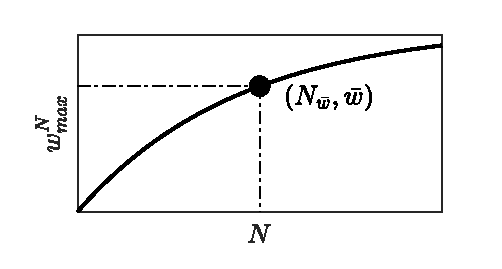
\includegraphics[scale = 0.85]{explain.eps}
			%\hspace{20pt}
			%\caption{An illustration of the bounds for the case of %$w_{\rm max}$ calculation. Any sequence %$||w(t)||_{\infty}=\bar{w}$ can drive $d_S(t)\geq %d_{S,{\rm max}}$ only after $k \geq N_{\bar{w}}$ of %application. We want to find the value of %$w^N_{max}=\bar{w}$ such that $N=N_{\bar{w}} \to \infty$. %This is $w_{\rm max}$. The analogous opposite applies to the %calculation of $w_{\rm min}$.   }
	%		\label{explanation}
	%	\end{center}
	%\end{figure} 
	%Any sequence $\{w(k)>w^N_{min},k=1:N\}$ will not drive $d_S(k \geq N)$ to the bound $d_{S,{\rm min}}$. Similarly, $\{w(k)<w^N_{max},k=1:N\}$ will not drive $d_S(k \geq N)$ to the bound $d_{S,{\rm max}}$. Hence, in order to explain the whole set $\mathcal{D}_{\infty}$, we need to find the lowest possible value of $w^N_{min}$ and the highest possible value of $w^N_{max}$ such that $d_S(k)$ is driven to its bounds in finite time $k$. This is achieved by increasing the value of $N$, which would require lower and higher values of $w(k)$ to make $d_S(N)$ reach $d_{S,{\rm min}}$ and $d_{S,{\rm max}}$ respectively. This leads to $w^N_{min}$ and $w^N_{max}$ asymptotically reaching their true values $w_{\rm min}$ and $w_{\rm max}$ as $N$ increases, thus making the set $\mathcal{W}_{\infty}$ completely explain the set $\mathcal{D}_{\infty}$.
	 %It is noted that the presented method provides a methodology to quantify uncertainty in any general ARX identified model.%

We remark that in practice the set $\mathcal{D}_{\infty}$ is constructed only based on a finite dataset $\hat{D}_{N}$ of $N$ samples. Consequently, the computation of the set $\mathcal{W}_{\infty}$ is also based  on a finite number of samples. Therefore, full robust
constraint satisfaction based on the sets $\mathcal{D}_{\infty}$ or $\mathcal{W}_{\infty}$
is only achieved asymptotically for $N=\infty$ samples
that capture all the possible values $d_S(t)$ can take.

\section{Case study}
	Numerical simulations are performed on a servo motor control problem, implementing the control scheme presented in Figure \ref{fullloop}. The sampling time is $T_s = 1 ms$. RMPC controllers are implemented for closed-loop models corresponding to both \eqref{TF_w} and \eqref{TF_d}. It is shown that using model \eqref{TF_w} results is superior performance, and hence performing an additional step to calculate $w_{\rm min}$ and $w_{\rm max}$ is justified.
	The simulations are implemented using MATLAB R2017b, with optimization problems occasionally implemented using YALMIP \cite{Lofberg2004}.
	\label{Case studies}
	%%%%%%%%%%%%%%%%%%%%%%%%%%%%%%%%%%%%%%%%%%%%%%%%%%%%%%
	\iffalse
	\subsection{Noise input bound}
	Consider a MISO system with inputs $\{u(t),w(t)\}$ and output $x(t)$, described by:
	\begin{equation*}
	\begin{matrix}
	u(t+1) = 0.995u(t)+1 \\
	x(t+1) = 0.05x(t)+u(t)+w(t) \\
	u(1) = 0, \hspace{5pt} x(1) = 0
	\end{matrix}
	\end{equation*}
	The input $u(t)$ is deterministic and $w(t)$ is the disturbance. An approximate ARX model of the system is calculated as $A(q^{-1})\tilde{x}(t) = B(q^{-1})u(t)+w(t)$ after performing experiments on the system and collecting data. It is identified with $A(q^{-1})$ and $B(q^{-1})$ having two and one free parameter each. Following this, the methodology discussed in Sect.\ref{Noise} is used to calculate bounds on $w(t)$.
	\\
	First, the signal $d_S(t)=x(t) - (B(q^{-1})/A(q^{-1}))u(t)$ is extracted from the experimental data, and $\mathcal{D}_{\infty}$ is constructed. For increasing values of $N$, sequences $\{w(k),k=1:N\}$ and corresponding $\{d_S(k),k=1:N\}$ are calculated by solving the optimization problems in \eqref{bound_problem}. The bounds $-\bar{w}_j(N)$ and $\bar{w}_j(N)$ on the input sequences are shown in Figure \ref{bounds}.
	The largest region where $-\bar{w}_j(N) \leq w(k) \leq -\bar{w}_j(N)$ is satisfied, is $\mathcal{W}_{\infty}$. 
		\begin{figure}[h!]
			\hspace{30pt}
			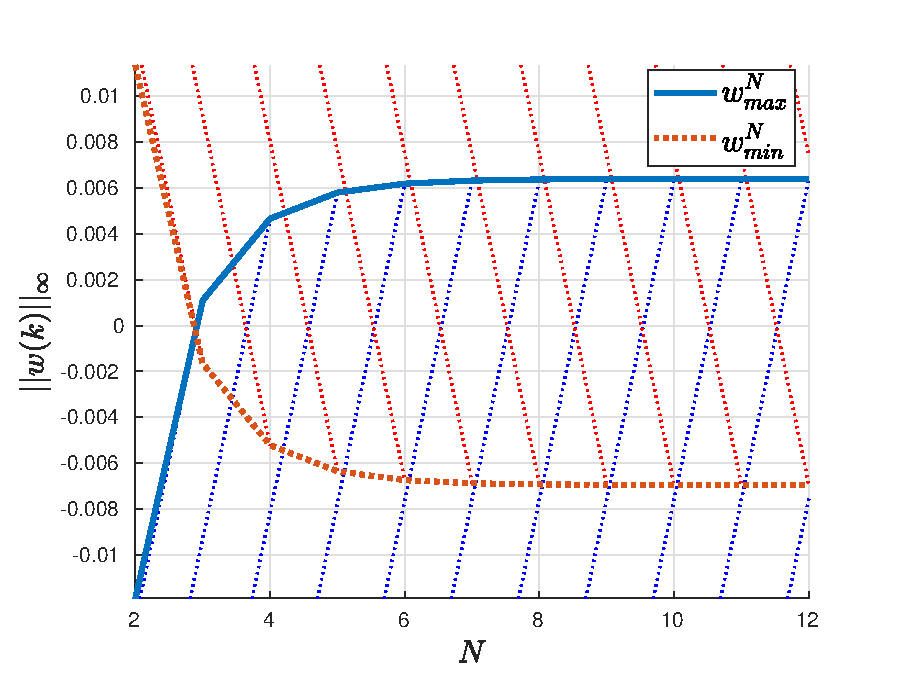
\includegraphics[scale = 0.60]{bounds.eps}
			\caption{Convergence of bounds to $w_{\rm min}$ and $w_{\rm max}$, with zero mean noise assumption.}
			\label{bounds}
		\end{figure} \vspace{-5pt}\\
	To verify the obtained bounds, the system identified through ARX identification is simulated with deterministic inputs $u(t)$, and a range of disturbance inputs $w(t)$ sampled from $\mathcal{W}_{\infty}$. The simulation results are seen in Figure \ref{simulation}. It can be seen that output of the ARX model simulated with noise inputs $w(t)$ covers the measurement range, and avoids conservatism. This is an indicator that the set $\mathcal{W}_{\infty}$ is valid.
	\begin{figure}[h]
		\hspace{22pt}
		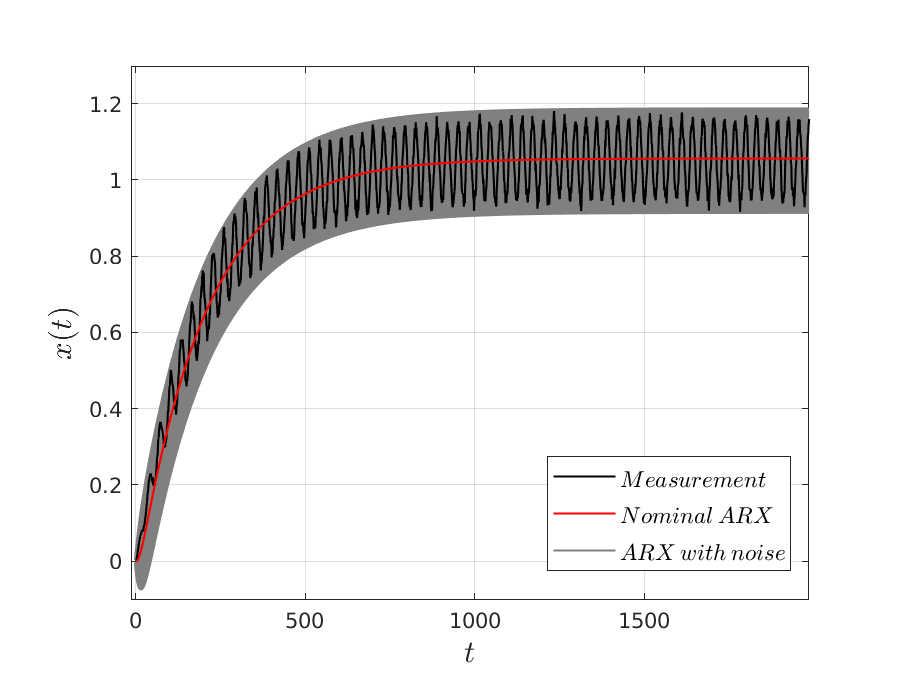
\includegraphics[scale = 0.70]{simulation.eps}
		\caption{Comparison of ARX model performance with constant $w(t)=0$(nominal) and $w(t)\in \mathcal{W}_{\infty}$. The appended disturbance model gives bounded output $x(t)$ without being conservative.}
		\label{simulation}
	\end{figure} 
	The simulation of ARX model with disturbance requires an initial condition on the disturbance model $\mathbb{D}_S$. In the current example, it is set to $0$. Since the actual initial condition of $\mathbb{D}_S$ might not be $0$, one might face problems with the model not covering the whole range of $\mathcal{D}_{\infty}$ during the transient period. To correct this, a state estimator could be used which rectifies the effect of initial state discrepancy, thus covering the noise effects even during transients.
	\fi
	%%%%%%%%%%%%%%%%%%%%%%%%%%%%%%%%%%%%%%%%%%%%%%%%%%%%%%
	\subsection{Robust data-driven MPC }
	The plant consisting of a servo positioning system is controlled using the scheme shown in Figure \ref{fullloop}. Plant dynamics are modeled by the following nonlinear state space equations:
	\begin{equation*}
	\small
	\begin{array}{rcl}
	\begin{bmatrix}
	\dot{\theta}(t) \vspace{12pt} \\
	\dot{\omega}(t) \vspace{12pt} \\
	\dot{i}(t)
	\end{bmatrix} &=& 
	\begin{bmatrix}
	\omega(t) \vspace{3pt}\\
	\cfrac{-mgl}{J}\hspace{1pt}sin\theta(t)-\cfrac{b}{J}\hspace{1pt}\omega(t) + \cfrac{K_m}{J}\hspace{1pt}i(t) \\  
	\cfrac{-K_m}{L}\hspace{1pt}\omega(t)-\cfrac{R}{L}\hspace{1pt}i(t) + \cfrac{1}{L}\hspace{1pt}u(t)
	\end{bmatrix} \vspace{10pt}\\
	y(t) &=& \begin{bmatrix} 1 & 0 & 0 \end{bmatrix} 
	\begin{bmatrix} \theta(t) \\ \omega(t) \\ i(t) \end{bmatrix} 
	\end{array}
	\end{equation*}
	\begin{table}[h!]
		\hspace{20pt}
		\begin{tabular}{||c|c|c||} 
			\hline
			Symbol & Parameter & Value\\ [0.5ex] 
			\hline\hline
			$R$ & Motor resistance & $5\Omega$ \\ 
			%\hline
			$L$ & Motor inductance & $5.10^{-3}$H \\
			%\hline
			$K_m$ & Motor torque constant & $0.0847$Nm/A \\
			%\hline
			$J$ & Complete disk inertia & $5.10^{-5}$Nm$^2$ \\
			%\hline
			$b$ & Friction coefficient & $3.10^{-3}$Nms/rad \\
			%\hline
			$m$ & Additional mass & $3$Kg \\
			%\hline
			$l$ & Mass offset & $2$m \\
			\hline
		\end{tabular}
		\caption{Physical parameters of servo motor system}
		\label{Simparam}
		\vspace{-10pt}  
	\end{table}
	\normalsize\\
	The states of the system $\theta(t)$, $\omega(t)$, and $i(t)$ are angle $[rad]$ and rotational velocity $[rad/s]$ of the servo motor, and armature current $[A]$ respectively. The input $u(t)$ is the voltage $[V]$ applied across the motor, and the output $y(t)$ is the rotational angle. 
	A VRFT methodology is used to design a stabilizing PD controller, which provides a voltage input $u(t)$ to make the rotational angle $y(t)$ track a reference signal $g(t)$. To this end, experiments are conducted with a low-pass filtered white noise signal $u(t)$ with a standard deviation of $10$V. The output angle $y(t)$ is recorded and the dataset $\mathbb{D}_N$ is obtained. A slow reference closed loop model $\mathbb{M}_P$ is chosen, given by:
	\begin{equation*}
	\begin{matrix}
	x_M(t+1) = 0.99x_M(t) + 0.01g(t)\\
	y_M(t) = x_M(t)
	\end{matrix}
	\end{equation*}
	The PD inner-loop controller $\mathbb{K}_P$ is parameterized as:
	\begin{equation*}
	u(t) = K_pe(t) + K_d\cfrac{e(t)-e(t-1)}{T_s}
	\end{equation*} 
	Solving the optimization problem \eqref{VRFT_problem}, the parameters 
	$K_p$ and $K_d$ are calculated using the dataset $D_N$. The controller is placed in the inner loop within the hierarchical control architecture.
	After VRFT synthesis, an outer MPC is designed using the formulation in \eqref{MPC}, to provide a reference signal $g(t)$. The output $y(t)$ is constrained to lie between $-1$ rad and $1$ rad, and the voltage input $u(t)$ between $-3.5$ V and $3.5$ V. An MPC horizon of $N_P=10$ timesteps is chosen, and weights are $Q_y=1$ and $Q_{\epsilon}=1$. \\
	Towards formulating the RMPC controller instead of the deterministic MPC controller, the disturbance model discussed in Sect. \ref{Contribution} is developed. First, the dataset $\hat{D}_N$ is built by performing closed loop experiments with input signal $\hat{g}(t)$ of standard deviation $10$ rad. Then, a linear model for $\mathbb{D}$ parameterized by $n_{a_D} = 4$ and $n_{b_D} = 3$ is identified by solving \eqref{DSensor}. Two equivalent models of the appended system, corresponding to \eqref{TF_w} and \eqref{TF_d}, are developed.  \\ 
	\indent For the model corresponding to \eqref{TF_w}, the disturbance model is split into two parts, $\mathbb{D}_D$ and $\mathbb{D}_S$, with inputs $g(t)$ and $w(t)$ respectively. Bounds on the exogenous disturbance $w(t)$ for a horizon $N$ are calculated by solving the linear problems \eqref{bound_problem}. The evolution of these bounds with increasing values of horizon $N$ is plotted in Figure \ref{bounds_RG}.  According to Theorem 1, the values $w_{\rm min}$ and $w_{\rm max}$ are obtained at convergence of  $\bar{w}_1(N)$ and $\bar{w}_2(N)$ respectively.
	\begin{figure}[h]
		\hspace{40pt}
		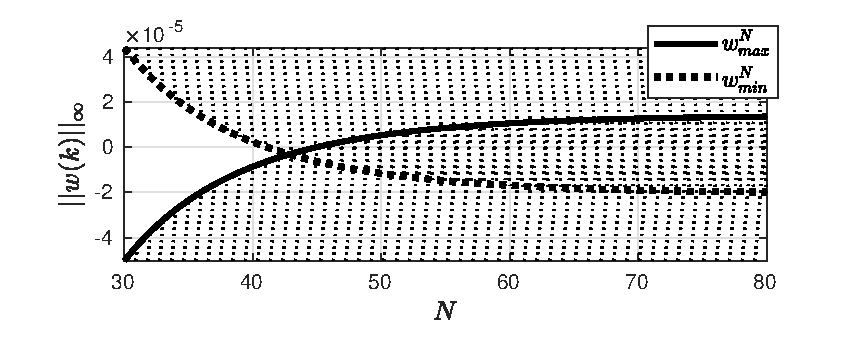
\includegraphics[scale = 0.50]{bounds_RG.eps}
		\caption{Convergence of bounds on $w(t)$ acting as input to the disturbance model $D_S$.}
		\label{bounds_RG}
	\end{figure} \\
	For the model corresponding to \eqref{TF_d}, the disturbance model consists of $\mathbb{D}_D$ and a direct exogenous disturbance signal $d_S(t)$. The bounds $d_{S,{\rm min}}$ and $d_{S,{\rm max}}$ on $d_S(t)$ are set equal to the minimum and maximum values of prediction error obtained during identification of the ARX model for $\mathbb{D}$ respectively. \\
	These models and related disturbance bounds are used in the formulation of corresponding RMPC controllers. To this end, constraints on the reference signal $g(t)$ are constructed, as shown in \eqref{MOAS}. At each time step $t$, the state vector $\gamma(t)$ is built with the assumption of no additional measurement noise. Solving the linear programs \eqref{RG_offline} till convergence to calculate the complete constraint set $\mathbb{G}_{\infty}(\gamma(t))$ can result in very conservative constraints on $g(t)$. This is avoided by solving them only for the duration of RMPC horizon by setting $k_c = N_P$. Since the bounds used for the calculation of constraint sets \eqref{MOAS} are calculated only based on a finite dataset $\hat{D}_{N}$ of size $N$, actual robustness is achieved only asymptotically for $N=\infty$ samples.\\
	Following this,
	the optimization problem \eqref{RMPC} is constructed and solved by the RMPC controller, generating a constraint satisfying reference signal $g(t)$.
	Performance of the control system for all these cases is plotted in Figure \ref{VRFT_y} and Figure \ref{VRFT_u}.
	\begin{figure}[t]
		\hspace{20pt}
		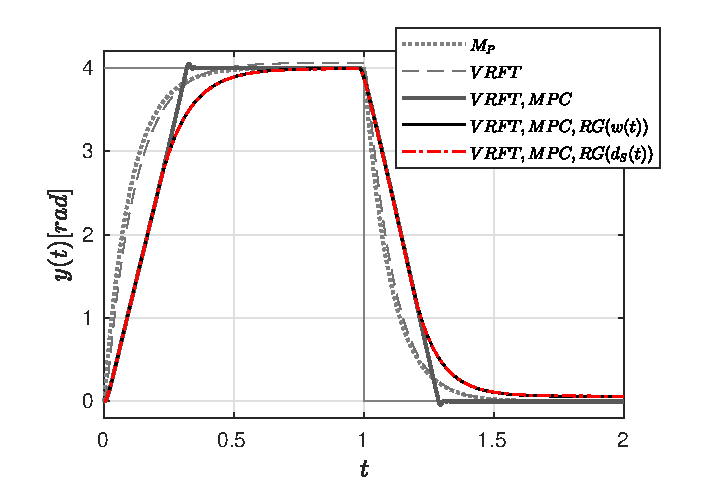
\includegraphics[scale = 0.50]{VRFT_vs_MPC.eps}
		\caption{The performance inner closed-loop does not exactly match the reference model $M_P$. MPC improves the performance but results in small constraint violation. Constraint violation is robustly avoided by using an RMPC controller instead of deterministic MPC. Using \eqref{TF_d} results in a conservative performance compared to \eqref{TF_w}.  }
		\label{VRFT_y}
	\end{figure} 
	\begin{figure}[t]
		\hspace{20pt}
		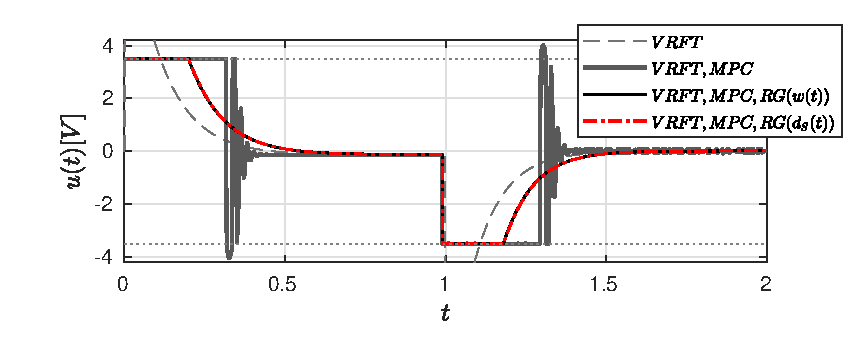
\includegraphics[scale = 0.50]{VRFT_vs_MPC_u.eps}
		\caption{Comparison of voltage input $u(t)$.}
		\label{VRFT_u}
	\end{figure} 
	It can clearly be seen that utilizing an RMPC controller instead of a deterministic MPC controller in the outer loop results in robust constraint satisfaction. Also, using the closed-loop model corresponding to \eqref{TF_d} as the plant model for RMPC controller design results in conservative performance when compared to using \eqref{TF_w}, for the same constraint set horizon $k_c = N_P$. Since the calculation of bounds $w_{\rm min}$ and $w_{\rm max}$ (which are required to use \eqref{TF_w} for RMPC synthesis) is performed offline, conservativeness of the control scheme can be reduced without any additional online operation. Note that increasing the constraint set horizon by solving \eqref{RG_offline} to convergence results in conservative performance from both the models, with \eqref{TF_w} still outperforming \eqref{TF_d}. 
	
	\section{Conclusion}
	This paper builds on the hierarchical data-driven control of constrained systems, by introducing robustness with respect to constraint satisfaction. This is done by using a robust model predictive controller.  Uncertainty on the model utilized by the RMPC controller is modeled as a disturbance input lying within an unknown bounded polyhedral set. 
	In this work, a novel technique to compute this polyhedral set from ARX identification is presented. It is seen that utilizing the model and the disturbance set calculated using the presented technique results in robust constraint satisfaction, all without identifying an open-loop model of the non-linear plant. Future work deals with extending the formulation to general Box-Jenkins models. Possible extensions to the control scheme include modifications to incorporate LPV systems.

	
                                                             
\bibliography{references}



\end{document}
